\section{Discontinuous Finite Element Discretization}    
\subsection{DFEM and sweeps}
Using \cref{transport_op,phi_D_psi}, \cref{one_speed} can be written:
\begin{align}
  &\(\bo_d \cdot \bn +\Sigma_t(\br)\)\psi_d = q(\br) \label{transport_op_2}\\
  &q(\br) = \frac{1}{4\pi}\Sigma_s(\br) \phi(\br) + \frac{1}{4\pi} S(\br).
  \label{tot_src}
\end{align}
$q(\br)$ is a volumetric source. For anisotropic scattering,
\cref{transport_op_2} would also include higher angular terms. During a sweep,
\cref{transport_op_2} is inverted.

Next, the domain $\mc{D}$ is meshed into elements $K$, $\psi_d$ is expanded on
the basis function $\chi_i$ ($\psi_d = \sum_i \psi_{d,i} \chi_i$),
\cref{transport_op_2} is multiplied by $\chi_j$, and \cref{transport_op_2} is
integrated over $K$:
\begin{equation}
  \int_K \(\bo_d \cdot \bn +\Sigma_t\) \(\sum_i \psi_{d,i}\chi_i\)\chi_j\
  d\br = \int_K \(\sum_i q_i\chi_i\) \chi_j\ d\br.
\end{equation}
Applying Stokes' theorem, we obtain:
\begin{equation}
  \begin{split}
    &\oint_{\partial K}\bo_d\cdot\bs{n}_b \(\sum_i\psi_{d,i}\chi_i\)\chi_j\ d\br -
    \int_K\(\sum_i\psi_{d,i}\chi_i\)\bo_d\cdot\bn\chi_j\ d\br+\\
    &\int_K \Sigma_t \(\sum_i \psi_{d,i}\chi_i\)\chi_j\ d\br = \int_K \(\sum_i
    q_i\chi_i\) \chi_j\ d\br
    \label{transport_weak}
  \end{split}
\end{equation}
where $\oint_{\partial K}$ is the integral over the boundary $\partial K$ and
$\bs{n}_b$ is the exterior normal.
Using upwind, \cref{transport_weak} becomes:
\begin{equation}
  \begin{split}
    &-\int_K \(\(\sum_i \psi_{d,i}\chi_i\) \bo_d \cdot \bn \chi_j +\Sigma_t
    \(\psi_{d,i} \chi_i\)\chi_j\)\br +\\
    &\int_{\partial K^+} \bo_d \cdot \bs{n}_b \(\sum_i \psi_{d,i} \chi_i\)
    \chi_j\ d\br = \int_K \(\sum_i q_i\chi_i\)\chi_j\ d\br +\\
    &\int_{\partial K^-} |\bo_d \cdot
    \bs{n}_b|\(\sum_i\psi_{d,i}^{\uparrow}\chi_i\)\chi_j\ d\br
  \end{split}
  \label{element_residual_formula}
\end{equation}
where $\partial K^-$ is the inflow of element $K$ $\(\bo_d \cdot \bs{n}_b
<0\)$ and $\partial K^+$ is the outflow face of element face
of element $K$ $\(\bo_d \cdot \bs{n}_b>0\)$. The angular flux values on an
inflow face, denoted by $\psi_d^{\uparrow}$ in
\cref{element_residual_formula}, are taken from the upwind neighbor element of
that face. We see that \cref{element_residual_formula} can be inverted for
only cell $K$ as soon as $\psi_d^{\uparrow}$ is known, yielding the concept of
transport sweep through the mesh.

\subsection{BiLinear Discontinous finite elements}
In this research, the BLD basis functions are used only on the rectangular
cells. If the cells are arbitrary convex quadrilateral, the discretization may
not exist (the system of equations obtained may be ill-conditioned). The BLD basis 
functions defined on the following rectangular cell:
\begin{figure}[H]
  \centering
  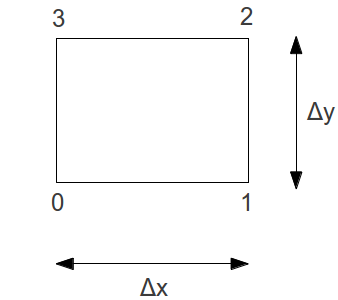
\includegraphics[width=0.2\textwidth]{./Spatial_discretizations/cell}
  \caption{Cell}
\end{figure}
are:
\begin{align}
  &\chi_0(x,y) = \frac{(\Delta x-x)}{\Delta x}\frac{(\Delta y-y)}{\Delta y}\\
  &\chi_1(x,y) = \frac{x}{\Delta x}\frac{(\Delta y-y)}{\Delta y}\\
  &\chi_2(x,y) = \frac{x}{\Delta x}\frac{y}{\Delta y}\\
  &\chi_3(x,y) = \frac{(\Delta x-x)}{\Delta x}\frac{y}{\Delta y}
\end{align}
with $x\in[0,\Delta x]$ and $y\in[0,\Delta y]$. On a square cell, the basis 
functions are given in Figure (\ref{bld}):
\begin{figure}[H]
\centering    
\subfloat[First basis function]{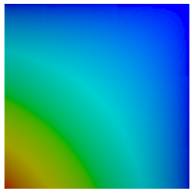
\includegraphics[width=0.25\textwidth]
  {./Spatial_discretizations/bld_1}}
\subfloat[Second basis function]{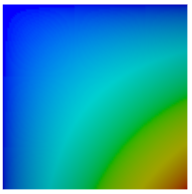
\includegraphics[width=0.25\textwidth]
  {./Spatial_discretizations/bld_2}}\\
\subfloat[Third basis function]{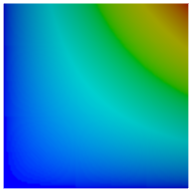
\includegraphics[width=0.25\textwidth]
  {./Spatial_discretizations/bld_3}}
\subfloat[Fourth basis function]{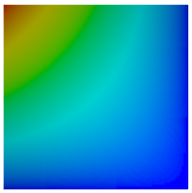
\includegraphics[width=0.25\textwidth]
  {./Spatial_discretizations/bld_4}}
\caption{BLD basis function}
\label{bld}
\end{figure}
Given these basis functions, the matrices of
\cref{element_residual_formula} (1D and 2D mass matrix, $\bs{M}_{ij} = \int_K
\chi_i \chi_j\ d\br$ and the ``gradient'' matrix, $\bs{G}_{ij} = \int_K \chi_i
\bn \chi_j\ d\br$) can be easily analytically computed on rectangular cells.
On ``almost'' rectangular cells, the integrals have to be computed
analytically. On highly distorted cells, these integrals become singular.
